\documentclass[]{article}

\usepackage{arxiv}
\usepackage[utf8]{inputenc} % allow utf-8 input
\usepackage[T1]{fontenc}    % use 8-bit T1 fonts
\usepackage{hyperref}       % hyperlinks
\usepackage{url}            % simple URL typesetting
\usepackage{booktabs}       % professional-quality tables
\usepackage{amsfonts}       % blackboard math symbols
\usepackage{nicefrac}       % compact symbols for 1/2, etc.
\usepackage{microtype}      % microtypography
\usepackage{lipsum}
\usepackage{graphicx}	% Including figure files
\usepackage{mathtools}  %loads amsmath as well
\usepackage{amssymb}	% Extra maths symbols
\usepackage[english]{babel}
\usepackage{float}
\usepackage{bm}
\usepackage{indentfirst}
\usepackage{tikz}
\usetikzlibrary{positioning}
\usepackage{pgfplots}
\usepackage{color,soul}
%\pgfplotsset{compat=1.12}
\definecolor{mygray}{RGB}{125,125,125}
\definecolor{myred}{RGB}{255,60,60}
\definecolor{myblue}{RGB}{60,60,255}
\renewcommand{\arraystretch}{1.2}

% potential journals:
    % journal of computational physics
    % computers and fluids
    % international journal for numerical methods in fluids
    % aiaa
    % journal of fluid mechanics


\title{Accelerating Block-Structured Adaptive Multiresolution Schemes: Applications to Reactive Flows}

\author{
  Brandon Gusto\\
  Department of Scientific Computing\\
  Florida State University\\
  Tallahassee, FL 32306 \\
  \texttt{bgusto@fsu.edu} \\
  %% examples of more authors
  \And
  Tomasz Plewa \\
  Department of Scientific Computing\\
  Florida State University\\
  Tallahassee, FL 32306 \\
  \texttt{tplewa@fsu.edu} \\
}

\begin{document}
\maketitle

\begin{abstract}
    We present a generalization of Harten's original multiresolution scheme for
    simulating reactive flows on logically rectangular block-structured adaptive
    mesh refinement (AMR) grids in one and two dimensions. The scheme addresses
    a major shortcoming of tree-based AMR codes, which is the creation of blocks
    with a low filling factor; that is, many cells in such a block are resolved
    beyond the desired error tolerance, necessitating excessive computational
    resources.  To overcome this issue, we introduce a multiresolution
    representation of the solution, not only to adapt the grid but also to
    adaptively compute fluxes and sources on each block. The scheme recycles
    regularity information obtained by the multiresolution grid adaptation in
    order to select flux and source calculations which may be accurately
    replaced by interpolation from the multiresolution basis. A block which
    employs this scheme is denoted as a fully adaptive block (FAB).  The error
    introduced by this approximation is shown to be of the same order as the
    local truncation error of the reconstruction scheme. Thus the rate of
    convergence of the underlying spatial reconstruction scheme is preserved.
    Additionally with respect to parallel applications, the multiresolution
    transform and computation of fluxes and sources on FABs is asynchronous,
    requiring only one synchronization step which is equivalent to the filling
    of ghost cells for each block. The efficiency of the scheme is demonstrated
    using several one and two-dimensional problems.
\end{abstract}

% keywords can be removed
\keywords{Multiresolution \and Adaptive Mesh Refinement \and Reactive Flows}

\section{Introduction}

    % paragraph introduces the need for spatially adaptive grids
    Highly energetic, reacting flows are characterized by disparate spatial and
    temporal length scales. Shock waves and burning fronts in the flow require
    orders of magnitude more resolution than smooth regions of the flow.
    Efficient simulation of such flows requires an adaptive strategy.

    % paragraph introducing adaptive mesh refinement as a concept
    The most popular strategy to accurately capture regions of interest in fluid
    simulations is to introduce a non-uniform spatial grid, with higher
    resolution near discontinuities or sharp gradients.  Methods which introduce
    a hierarchy of nested grid resolutions are generally described as adaptive
    mesh refinement (AMR) methods. AMR methods, first introduced in
    \cite{berger1984}, usually rely on estimates of the local truncation error
    (LTE) of the numerical scheme to determine regions where refinement is
    necessary for solution accuracy. Some more simple strategies may refine
    based on the value of the gradient, or concentration of some species of
    interest. For a full review of the LTE estimators and refinement criterion,
    readers are referred to \hl{blank}.

    % talk about block-structured AMR
    Regarding the implementation of AMR methods on large networks of parallel
    computers, certain engineering realities have neccessitated the reduction in
    granularity of the adaptive refinement. To use a single computational cell
    as the unit for refinement (i.e. cell-based refinement) introduces a number
    of costly compromises. Firstly, such an adapted grid requires the
    reconstruction method of choice to utilize nonuniform stencils, requiring
    increased computational resources. More significantly, the cell-based
    refinement requires costly data traversal. Traversing tree space requires on
    average $\mathcal{O}(n^d)$ (\hl{confirm this?}) operations, where $n$ is the
    number of cells per dimension, $d$. Thus most AMR codes make use of some
    type of block-based approach. Tree-based block-structured codes, where each
    block consists of a fixed number of cells, are a very popular choice. These
    types of approaches are implemented in a number of AMR libraries including
    Paramesh (\hl{cite}), p4est (\hl{cite}, and others. This approach allows for
    simple mesh management procedures, and scales well for very large numbers of
    processors in parallel.  One clear drawback however is the gradedness of the
    tree, which necessitates that no branch can have an incomplete set of
    children. This typically leads to refinement of many blocks which would not
    be otherwise flagged by refinement indicators. A further complication
    imposed by most finite volume solvers is that there can not be a jump in
    refinement greater than one level. Together these consequences of AMR
    represent a non-trivial decrease in performance due to the fact that the
    mesh is not optimal (in some sense).
e
    % paragraph reviews the work of harten and multiresolution methods
    Alternate approaches to dynamic grid adaptation based on wavelet theory
    became popular after the seminal papers by Harten \cite{harten1994}, were
    introduced. In this work, a multiresolution representation of the discrete
    solution on a uniform grid was used for adaptively computing the divergence
    of the flux within a finite volume framework. Rather than adapt the grid
    directly, the idea was to accelerate the computation of fluxes using the
    multiresolution information. In this approach, eligible fluxes in
    sufficiently smooth regions are interpolated from fluxes obtained at
    interfaces corresponding to coarser grid levels. The original scheme was
    applied solely to hyperbolic conservation laws in one spatial dimension, but
    was then expanded by Bihari et. al. to two-dimensional simulations in
    (\hl{citation}), followed by the inclusion of viscous terms in
    (\hl{citation}), and then to source terms in the context of reactive flows
    in (\hl{bihari}). These works retained the original spirit of Harten's
    scheme, which was to evolve the solution on a uniform grid, but use
    multiresolution information to identify regions where flux (and/or source
    term) computations may be avoided.

    % review the multiresolution-adaptive papers
    Although Harten's original scheme was intended to be an alternative to
    spatially non-uniform grid adaptation, a series of papers have since
    reintroduced the concept of non-uniform grids within the MR framework. Thus
    the AMR approach was essentially redeveloped but with the refinement
    criterion defined by the MR representation rather than with the traditional
    metrics mentioned previously. The first fully adaptive scheme was presented
    by Cohen et. al. to study hyperbolic conservation laws in two dimensions in
    (\hl{cite}). More recently, Rossinilli et. al. explored the use of
    wavelet-based refinement indicators for block-based adaptation.

    % punchline
    In the following work, we present a novel block-based adaptive mesh
    refinement scheme using wavelet-based indicators, where Harten's scheme is
    used to essentially treat each block as a uniform grid.  The indicators are
    used for two purposes: (1) refinement, and (2) adaptively calculating fluxes
    and source terms. We show how this scheme costs essentially nothing in
    additional computation (the MR information is recycled after adaptation),
    while not impacting the accuracy of the solver.

    In the section 2 of this manuscript, we describe the conservations laws
    of interest as well as the underlying finite volume
    method and discretization. In section 3, we introduce the multiresolution
    decomposition of the numerical solution. In section 4, the block-based
    adaptive scheme is introduced, which combines grid adaptation with the
    interpolatory scheme of Harten \hl{cite}.

\section{Finite volume method}

    % introduce conservation laws
    In the present work we are interested in numerically solving conservation
    laws of the form
    \begin{equation}
    \begin{cases}
      u_{t} + \nabla \cdot f(u) = s(u) \\
      u(x,0) = u_{0}(x).
    \end{cases}
    \label{claw}
    \end{equation}
    where $u \in \mathbb{R}^{m}, x \in \mathbb{R}^{n},$ and $t > 0$. Here
    $u(t,x)$ represents a conserved quantity, $f(u)$ is the flux function, and
    $s(u)$ is a source term. \hl{Discuss discontinuous solutions}.

    In the finite volume formulation, the spatial domain is discretized into
    control volumes $V_{i}$, inside which the solution is approximated by volume
    averages as
    \begin{equation}
        \overline{u}_{i}(t) = \frac{1}{|V_{i}|} \int_{V_{i}} u(x,t) dx.
    \end{equation}
    The governing equations are cast into the semi-discrete conservative form
    by application of the divergence theorem, yielding
    \begin{equation}
        \frac{d \overline{u}_{i}(t)}{dt} = L(\overline{u}) =  -\frac{1}{|V_{i}|} \sum_{j} |
        \Gamma_{i,j}| \hat{f}_{i,j}
        + \overline{s}_{i},
        \label{ode}
    \end{equation}
    where interfaces are represented as $\Gamma_{i,j} = V_{i} \cap
    V_{j}$. The sources are given in a cell-averaged sense as
    \begin{equation}
        \overline{s}_{i} = \frac{1}{|V_{i}|} \int_{|V_{i}|} s(u) dx,
    \end{equation}
    and the numerical flux is evaluated as
    \begin{equation}
        \hat{f}_{i,j} = \hat{f}(u^{-}_{i,j}, u^{+}_{i,j}),
    \end{equation}
    where the states $u^{-}_{i,j}$ and $u^{+}_{i,j}$ indicate the approximate
    value of the quantity $u$ on opposite sides of the cell
    interface $\Gamma_{i,j}$.

    %These values are reconstructed from a stencil of
    %cell averages using weighted essentially non-oscillatory schemes of
    %variable order.

    \subsection{Spatial reconstruction and calculation of fluxes}

        % overview of PPM
        In the vast majority of multiresolution finite volume schemes
        introduced in the previously mentioned works, the reconstruction
        methods of choice belong to the class of essentially non-oscillatory
        (ENO) or weighted ENO (WENO) schemes. For flows exhibiting strong
        shocks and contact discontinuities, the higher-order WENO schemes
        generally do not reap additional benefit (\hl{citation and also Tomek
        can provide input here?}). In the present work, we use the piecewise
        parabolic method (PPM) of Woodward and Collela \hl{ref} to reconstruct
        the field and provide left and right inputs to the Riemann solver at
        each cell interface. \hl{More here from Tomek}.

    \subsection{Time integration}

        % define evolution operator as in domingues2008
        Once the system of ordinary differential equations (\ref{ode}) is
        constructed, the objective is to integrate them forward in time. In our
        implementation we use a second-order explicit TVD Runge-Kutta scheme to
        advance. This is summarized by
        \begin{align}
            & \tilde{\bm{u}}_{1} = \bm{u}^{n} + c_{1} \Delta t L(\bm{u}^{n}) \\
            & \tilde{\bm{u}}_{2} = \tilde{\bm{u}}_{1} + c_{2} \Delta t L(\tilde{\bm{u}}_{1}) \\
            & \bm{u}^{n+1} = b_{1} \tilde{\bm{u}}_{1} + b_{2} \tilde{\bm{u}}_{2}.
        \end{align}

\section{Adaptive multiresolution scheme on a uniform grid}

    % describe overview of transform, and average-interpolating wavelets
    We present here a brief review of the multiresolution concepts, as first
    introduced by Harten \hl{cite} within the context of conservative finite
    volume schemes. The scope here is restricted to one-dimensional uniform
    grids, as the operations required for the fully adaptive block scheme are
    identical.

    \subsection{Reference scheme on one-dimensional uniform grid}

    On a one-dimensional uniform grid, the evolution equation \ref{ode} becomes
    \begin{equation}
        \frac{d \overline{u}_{i}(t)}{dt} = -\frac{1}{\Delta x} \left( \hat{f}_{i+1/2} -
        \hat{f}_{i-1/2} \right) + \overline{s}_{i},
        \label{ode}
    \end{equation}
    where the subscripts $i-1/2$, $i+1/2$ denote the left and right interfaces, respectively.

    \subsection{Multiresolution representation of data}

    The multiresolution approach decomposes data by introducing a hierarchy
    of nested discretizations, $\bm{\mathcal{G}}_{l}$. The objective of the
    multiresolution procedure is to represent the fine-grid data as a sum of
    values at the coarsest level plus a series of differences at finer levels.
    The result is a decomposition which provides frequency and scale
    information of the underlying data.

    The grids are defined by
    \begin{equation}
        \bm{\mathcal{G}}_{l} = \left\{ x_{i}^{l} \right\}_{i=0}^{N_{l}}, \text{ }
        \text{ } \text{ } \text{ } x_{i}^{l} = i \cdot \Delta x_{l}, \text{ }
        \text{ } \Delta x_{l} = 2^{L-l} \cdot \Delta x_{L}, \text{ } \text{ } N_{l} = N_{L}
        / 2^{L-l},
    \end{equation}
    where $\Delta x_{l}$ and $N_{l}$ denote the cell width and number of cells,
    respectively, on level $l$. The index space of cells on each level of the
    hierarchy is denoted by $\bm{\mathcal{I}}^{l} = \left\{ 1,\dots,N_{l}
    \right\}$ Given cell averages at the finest resolution,
    $\bm{\overline{u}}^{L}$, the forward transform proceeds by performing the
    following set of mappings on levels $l = L-1,L-2,\dots,1$:
    \begin{enumerate}
        \item[] \textit{Project:} The cells at level $l+1$ are projected
            by means of averaging, onto the coarser grid
            level $l$. The projection is defined by a linear operator
            which performs the mapping $\bm{P}_{l+1}^{l} : \overline{\bm{u}}^{l+1}
            \mapsto \overline{\bm{u}}^{l}$.
        \item[] \textit{Predict}: Cell averages at level $l+1$
            are predicted by an average-interpolating polynomial constructed
            of cells on level $l$. The prediction operator performs
            the mapping $\bm{P}_{l}^{l+1} : \overline{\bm{u}}^{l} \mapsto
            \tilde{\bm{u}}^{l+1}$.
    \end{enumerate}
    The projection operation, which preserves averages at the finer level
    by design, is the simple weighted average of parent cells.  In one
    dimension, this average is given by
    \begin{equation}
        \overline{u}^{l}_{i} = \left( \bm{P}_{l+1}^{l}
        \overline{\bm{u}}^{l+1} \right)_{i} = \frac{1}{2} (
        \overline{u}^{l+1}_{2i-1} + \overline{u}^{l+1}_{2i} ), \quad \forall
        i \in \bm{\mathcal{I}}^{l}.
    \end{equation}
    The prediction operator is defined by a unique average-interpolating
    polynomial to predict, based on a stencil of cell averages at grid level
    $l-1$, the odd cell averages at the finer level $l$. The prediction
    mapping is performed using the following centered interpolants with
    $m\in\{0,1\}$,
    \begin{align}
%            \tilde{u}_{i}^{l} = \left( \bm{P}_{l-1}^{l} \bm{u}^{l-1}
%            \right)_{i} =
%            \begin{cases}
%                u_{i/2}^{l-1} - \sum_{p=1}^{s} \gamma_{p} \left( u^{l-1}_{i/2+p} -
%                u^{l-1}_{i/2-p} \right), \text{ } \text{ } \text{ } \forall
%                i \in \bm{\mathcal{I}}_{even}^{l} \\
%                u_{(i+1)/2}^{l-1} + \sum_{p=1}^{s} \gamma_{p} \left(
%                u^{l-1}_{(i+1)/2+p} - u^{l-1}_{(i+1)/2-p} \right), \text{ }
%                \text{ } \text{ } \forall i \in \bm{\mathcal{I}}_{odd}^{l}
%            \end{cases}
        \tilde{u}_{2i-m}^{l+1} = u_{i}^{l} - (-1)^{m} \sum_{p=1}^{s} \gamma_{p} \left(
            u^{l}_{i+p} - u^{l}_{i-p} \right), \quad \forall i \in \bm{\mathcal{I}}^{l}
        \label{prediction}
    \end{align}
    The coefficients $\gamma_{i}$ are supplied in Table (\ref{coeff1}). The
    order of accuracy of each interpolant is $r=2s+1$. Once the prediction is
    made, the difference information is obtained by computing the detail
    coefficients as
    \begin{equation}
        d^{l}_{i} = u^{l+1}_{2i} - \tilde{u}^{l+1}_{2i}, \quad \forall i \in \bm{\mathcal{I}}^{l}.
    \end{equation}
    The forward transform is complete when the detail coefficients have been
    computed on all levels $l=1,\dots,L-1$. The result of the forward
    transform operation can be succinctly written as
    \begin{equation}
        \bm{u}^{L}_{M} = \bm{M} \bm{u}^{L} = \left( \bm{d}^{L-1}, \bm{d}^{L-2},
        \dots, \bm{d}^{1}, \bm{u}^{1} \right)^{T},
    \end{equation}
    where $M$ denotes the linear transform operator, and $\bm{d}^{l} =
    \left\{d^{l}_{i}\right\}_{i=1}^{N_{l}}$.

    \subsection{Truncation}

        % describe truncation proceudure
        Once the difference information has been computed, compression of the
        fine-grid cell averages $\bm{u}^{L}$ is obtained by truncating
        coefficients whose magnitude is below a prescribed level-dependent
        threshold, $\varepsilon_{l}$.  In \cite{harten1994} the following
        threshold is proposed
        \begin{equation}
            \varepsilon_{l} = \varepsilon_{L} / 2^{L-l},
        \end{equation}
        where $\varepsilon_{L}$ is the tolerance prescribed for the finest
        level, naturally.  The detail coefficients are truncated according to
        \begin{equation}
            \tilde{d}^{l}_{i} =
                \begin{cases}
                    d^{l}_{i}, \text{ } \text{if} \text{ } |d^{l}_{i}| > \varepsilon_{l} \\
                    0, \text{ } \text{if} \text{ } |d^{l}_{i}| \leq
                    \varepsilon_{l},
                \end{cases}
        \end{equation}
        producing the following approximate representation,
        \begin{equation}
            \tilde{\bm{u}}^{L}_{M} = T_{\varepsilon}(\bm{u}^{L}_{M}) = \left(
            \tilde{\bm{d}}^{L-1}, \tilde{\bm{d}}^{L-2},
            \dots, \tilde{\bm{d}}^{1}, \bm{u}^{1} \right)^{T}.
        \end{equation}

%    \subsection*{Decoding}
%
%        % describe decoding
%        The fine-grid solution is reconstructed by computing from levels
%        $l=1,\dots,L-1$ the following
%s        \begin{align}
%s            u_{2i}^{l+1} & = d_{i}^{l} + \tilde{u}_{2i}^{l+1} \\
%s            u_{2i-1}^{l+1} & = 2 u_{i}^{l} - u_{2i}^{l+1},
%s        \end{align}
%s        for each cell on the level.  If the detail coefficients are truncated
%s        below a nonzero $\varepsilon$, the discrete representation becomes
%s        \begin{equation}
%s            \bm{u}^{L}_{\varepsilon} \approx \bm{M}^{-1} \tilde{\bm{u}}^{L}_{M}.
%s        \end{equation}

    \subsection{Adaptive calculation of fluxes}

        % dicuss computation of fluxes and sources
        Once the detail coefficients have been obtained, the MR scheme
        proceeds by setting a threshold $\varepsilon$ and truncating coefficients
        which have an absolute value below the threshold. Lastly, the inverse
        transform then starts from grid $l=L$ and at each interface either
        computes fluxes using the fine-grid scheme, or interpolates them using
        the MR basis. The fluxes are interpolated by
        \begin{equation}
            \hat{f}_{2i+1}^{l+1} \approx \sum_{p=1}^{s+1} \beta_{p} \left(
            \hat{f}^{l}_{i-p+1} + \hat{f}^{l}_{i+p} \right),
        \end{equation}
        where the interpolants are of degree $2s+1$. The coefficients for
        various degrees of polynomial interpolants are shown in Table (ref).
        The process repeats until all fluxes are either computed or
        interpolated on the fine grid $l=0$.

    \subsection{Adaptive calculation of source terms}

        % describe adaptive calculation of sources
        To reduce the cost of calculating source terms for reactive flows, we employ
        the same multiresolution procedure. For each cell which is not in the mask,
        we compute its children using the same operator as in \ref{prediction}.
        We compute
        \begin{equation}
            \overline{s}_{i}^{l+1} \approx \left( \bm{P}_{l}^{l+1} \bm{s}^{l}
                \right)_{i}, \text{ } \text{ } \text{ } \forall i \in
                \bm{\mathcal{I}}^{l+1}.
        \end{equation}

\section{Fully adaptive block-structured multiresolution scheme}

    % Key ideas: Perhaps we can utilize scale-selective WENO weights as in
    % maulik 2018. If the error is below threshold, skip the rieman solve altogether
    % and interpolate the flux based on harten's method. Also, explore
    % possibility of using WENO interpolation for the Harten flux interpolation near
    % boundaries? Actually probably not really necessary because the
    % approximation still preserves the same order.

%    \subsection*{Block-structured mesh adaptation}
%    % two main issues: no jump greater than one refinement level, and no
%    % incomplete trees
%    We define a mask $\bm{\mathcal{M}}(\varepsilon)$.
%
%    % illustration of parallel encoding
%    \begin{figure}[H]
%        \center
%        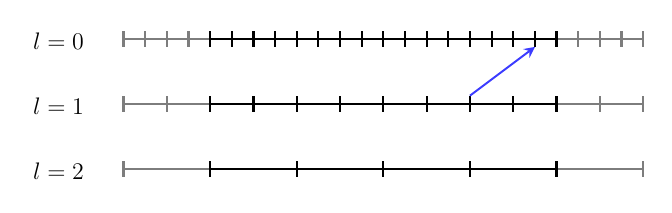
\begin{tikzpicture}[thick,scale=0.275, every node/.style={scale=0.6}]

    % variables
    \def\xl{-8.0}
    \def\xr{8.0}
    \def\y{0.0}
    \def\yy{-3.0}
    \def\yyy{-6.0}
    \def\ts{0.75}
    \def\op{0.35}
    \def\fx{0.15}
    
    % draw ghost cells
    \draw [mygray] (\xl-4,\y+\ts/2) --(\xr+4,\y+\ts/2);
    \draw [mygray] (\xl-4,\yy+\ts/2) --(\xr+4,\yy+\ts/2);
    \draw [mygray] (\xl-4,\yyy+\ts/2) --(\xr+4,\yyy+\ts/2);
    \draw [mygray] (\xl-1.0,\y) --(\xl-1.0,\y+\ts);
    \draw [mygray] (\xr+1.0,\y) --(\xr+1.0,\y+\ts);
    \draw [mygray] (\xl-2.0,\y) --(\xl-2.0,\y+\ts);
    \draw [mygray] (\xr+2.0,\y) --(\xr+2.0,\y+\ts);
    \draw [mygray] (\xl-3.0,\y) --(\xl-3.0,\y+\ts);
    \draw [mygray] (\xr+3.0,\y) --(\xr+3.0,\y+\ts);
    \draw [mygray] (\xl-4.0,\y) --(\xl-4.0,\y+\ts);
    \draw [mygray] (\xr+4.0,\y) --(\xr+4.0,\y+\ts);

    % ghost cells at level l=1
    \draw [mygray] (\xl-2.0,\yy) --(\xl-2.0,\yy+\ts);
    \draw [mygray] (\xr+2.0,\yy) --(\xr+2.0,\yy+\ts);
    \draw [mygray] (\xl-4.0,\yy) --(\xl-4.0,\yy+\ts);
    \draw [mygray] (\xr+4.0,\yy) --(\xr+4.0,\yy+\ts);

    % level l=2
    \draw [mygray] (\xl-4.0,\yyy) --(\xl-4.0,\yyy+\ts);
    \draw [mygray] (\xr+4.0,\yyy) --(\xr+4.0,\yyy+\ts);

    % draw grids
    \draw (\xl,\y+\ts/2) --(\xr,\y+\ts/2);
    \draw (\xl,\yy+\ts/2) --(\xr,\yy+\ts/2);
    \draw (\xl,\yyy+\ts/2) --(\xr,\yyy+\ts/2);
    
    % draw cells for max level
    \draw (\xl,\y) --(\xl,\y+\ts);
    \draw (\xl+1.0,\y) --(\xl+1.0,\y+\ts);
    \draw (\xl+2.0,\y) --(\xl+2.0,\y+\ts);
    \draw (\xl+3.0,\y) --(\xl+3.0,\y+\ts);
    \draw (\xl+4.0,\y) --(\xl+4.0,\y+\ts);
    \draw (\xl+5.0,\y) --(\xl+5.0,\y+\ts);
    \draw (\xl+6.0,\y) --(\xl+6.0,\y+\ts);
    \draw (\xl+7.0,\y) --(\xl+7.0,\y+\ts);
    \draw (\xl+8.0,\y) --(\xl+8.0,\y+\ts);
    \draw (\xl+9.0,\y) --(\xl+9.0,\y+\ts);
    \draw (\xl+10.0,\y) --(\xl+10.0,\y+\ts);
    \draw (\xl+11.0,\y) --(\xl+11.0,\y+\ts);
    \draw (\xl+12.0,\y) --(\xl+12.0,\y+\ts);
    \draw (\xl+13.0,\y) --(\xl+13.0,\y+\ts);
    \draw (\xl+14.0,\y) --(\xl+14.0,\y+\ts);
    \draw (\xl+15.0,\y) --(\xl+15.0,\y+\ts);
    \draw (\xl+16.0,\y) --(\xl+16.0,\y+\ts);
    
    % lower level cells
    \draw (\xl,\yy) --(\xl,\yy+\ts);
    \draw (\xl+2.0,\yy) --(\xl+2.0,\yy+\ts);
    \draw (\xl+4.0,\yy) --(\xl+4.0,\yy+\ts);
    \draw (\xl+6.0,\yy) --(\xl+6.0,\yy+\ts);
    \draw (\xl+8.0,\yy) --(\xl+8.0,\yy+\ts);
    \draw (\xl+10.0,\yy) --(\xl+10.0,\yy+\ts);
    \draw (\xl+12.0,\yy) --(\xl+12.0,\yy+\ts);
    \draw (\xl+14.0,\yy) --(\xl+14.0,\yy+\ts);
    \draw (\xl+16.0,\yy) --(\xl+16.0,\yy+\ts);
    
    % even lower level cells
    \draw (\xl,\yyy) --(\xl,\yyy+\ts);
    \draw (\xl+4.0,\yyy) --(\xl+4.0,\yyy+\ts);
    \draw (\xl+8.0,\yyy) --(\xl+8.0,\yyy+\ts);
    \draw (\xl+12.0,\yyy) --(\xl+12.0,\yyy+\ts);
    \draw (\xl+16.0,\yyy) --(\xl+16.0,\yyy+\ts);
 
    % arrows indicating flux interpolation dependency
    \draw[myblue,->,line width=0.25mm,>=stealth] (\xr-4,\yy+\ts) -- (\xr-1,\y);

    % nodes
    \node at (\xl-7.0,\y+0.25) {\Large $l=0$};
    \node at (\xl-7.0,\yy+0.25) {\Large $l=1$};
    \node at (\xl-7.0,\yyy+0.25) {\Large $l=2$};

\end{tikzpicture}

%        \caption{A block of consisting of $N^{0} = 16$ cells is shown. Four
%        ghost cells are included on each end of the block, allowing the
%        multiresolution decomposition to descend two levels (to grid level
%        $l=2$). Interpolation stencils for the computation of detail
%        coefficients at levels $l=1, l=2$ are shown, indicating the need for ghost cells.}
%    \end{figure}
%    % illustration amr block tree structure
%    \begin{figure}[H]
%        \center
%        \begin{tikzpicture}[sibling distance=2em,every node/.style = {shape=rectangle,align=center,top color=white}]

    % variables
    \def\y{0.0}
    \def\yy{-1.0}
    \def\yyy{-2.0}

    % label levels
    \node at (-2,\y) {$l=1$};
    \node at (-2,\yy) {$l=2$};

    % draw amr blocks
    \draw [thick] (0,\y) rectangle (5,\y);
    \draw [thick] (0,\y-0.1) rectangle (0,\y+0.1);
    \draw [thick] (5,\y-0.1) rectangle (5,\y+0.1);

    \draw [thick] (0,\yy) rectangle (5,\yy);
    \draw [thick] (0,\yy-0.1) rectangle (0,\yy+0.1);
    \draw [thick] (5,\yy-0.1) rectangle (5,\yy+0.1);
    \draw [thick] (2.5,\yy-0.1) rectangle (2.5,\yy+0.1);

    \draw [thick] (2.5,\yyy) rectangle (5,\yyy);
    \draw [thick] (3.75,\yyy-0.1) rectangle (3.75,\yyy+0.1);
    \draw [thick] (2.5,\yyy-0.1) rectangle (2.5,\yyy+0.1);
    \draw [thick] (5,\yyy-0.1) rectangle (5,\yyy+0.1);

    % block labels
    \node [shape=rectangle,align=center] at (2.5,\y) {1};
    \node [shape=rectangle,align=center] at (1.25,\yy) {2};

    % draw tree
    \node at (9,\y) {1}
        child { node {2} }
        child { node {3}[sibling distance=2em,every node/.style = {shape=rectangle,align=center,top color=white}]
            child { node {4} }
            child { node {5} } };

\end{tikzpicture}

%        \caption{}
%    \end{figure}
%
%    % pseudocode of algorithm
%
%    % illustration of parallel issue
%    \begin{figure}[H]
%        \center
%        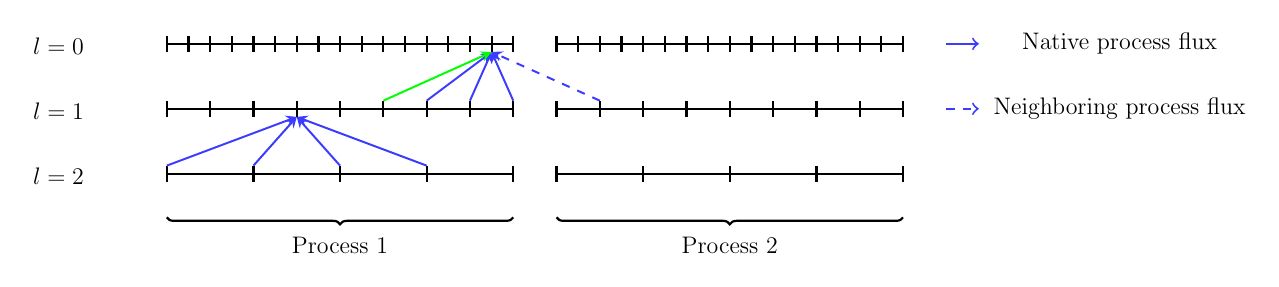
\begin{tikzpicture}[thick,scale=0.275, every node/.style={scale=0.6}]

    % variables
    \def\xl{-8.0}
    \def\xr{8.0}
    \def\y{0.0}
    \def\yy{-3.0}
    \def\yyy{-6.0}
    \def\ts{0.75}
    \def\op{0.35}
    \def\fx{0.15}
    
    % draw grids
    \draw (\xl,\y+\ts/2) --(\xr,\y+\ts/2);
    \draw (\xl,\yy+\ts/2) --(\xr,\yy+\ts/2);
    \draw (\xl,\yyy+\ts/2) --(\xr,\yyy+\ts/2);
    
    % draw cells for max level
    \draw (\xl,\y) --(\xl,\y+\ts);
    \draw (\xl+1.0,\y) --(\xl+1.0,\y+\ts);
    \draw (\xl+2.0,\y) --(\xl+2.0,\y+\ts);
    \draw (\xl+3.0,\y) --(\xl+3.0,\y+\ts);
    \draw (\xl+4.0,\y) --(\xl+4.0,\y+\ts);
    \draw (\xl+5.0,\y) --(\xl+5.0,\y+\ts);
    \draw (\xl+6.0,\y) --(\xl+6.0,\y+\ts);
    \draw (\xl+7.0,\y) --(\xl+7.0,\y+\ts);
    \draw (\xl+8.0,\y) --(\xl+8.0,\y+\ts);
    \draw (\xl+9.0,\y) --(\xl+9.0,\y+\ts);
    \draw (\xl+10.0,\y) --(\xl+10.0,\y+\ts);
    \draw (\xl+11.0,\y) --(\xl+11.0,\y+\ts);
    \draw (\xl+12.0,\y) --(\xl+12.0,\y+\ts);
    \draw (\xl+13.0,\y) --(\xl+13.0,\y+\ts);
    \draw (\xl+14.0,\y) --(\xl+14.0,\y+\ts);
    \draw (\xl+15.0,\y) --(\xl+15.0,\y+\ts);
    \draw (\xl+16.0,\y) --(\xl+16.0,\y+\ts);
    
    % lower level cells
    \draw (\xl,\yy) --(\xl,\yy+\ts);
    \draw (\xl+2.0,\yy) --(\xl+2.0,\yy+\ts);
    \draw (\xl+4.0,\yy) --(\xl+4.0,\yy+\ts);
    \draw (\xl+6.0,\yy) --(\xl+6.0,\yy+\ts);
    \draw (\xl+8.0,\yy) --(\xl+8.0,\yy+\ts);
    \draw (\xl+10.0,\yy) --(\xl+10.0,\yy+\ts);
    \draw (\xl+12.0,\yy) --(\xl+12.0,\yy+\ts);
    \draw (\xl+14.0,\yy) --(\xl+14.0,\yy+\ts);
    \draw (\xl+16.0,\yy) --(\xl+16.0,\yy+\ts);
    
    % even lower level cells
    \draw (\xl,\yyy) --(\xl,\yyy+\ts);
    \draw (\xl+4.0,\yyy) --(\xl+4.0,\yyy+\ts);
    \draw (\xl+8.0,\yyy) --(\xl+8.0,\yyy+\ts);
    \draw (\xl+12.0,\yyy) --(\xl+12.0,\yyy+\ts);
    \draw (\xl+16.0,\yyy) --(\xl+16.0,\yyy+\ts);
    
    % curly brace
    \draw[decoration={brace,mirror,raise=5pt},decorate]
        (\xl,\yyy-1.0) -- node[below=10pt] {\Large Process 1}(\xr,\yyy-1.0);

    % arrows indicating flux interpolation dependency
    \draw[myblue,->,line width=0.25mm,>=stealth] (\xr-4,\yy+\ts) -- (\xr-1,\y);
    \draw[myblue,->,line width=0.25mm,>=stealth] (\xr-2,\yy+\ts) -- (\xr-1,\y);
    \draw[myblue,->,line width=0.25mm,>=stealth] (\xr,\yy+\ts) -- (\xr-1,\y);
    \draw[myblue,dashed,->,line width=0.25mm,>=stealth] (\xr+4,\yy+\ts) -- (\xr-1,\y);
    \draw[green,->,line width=0.25mm,>=stealth] (\xr-6,\yy+\ts) -- (\xr-1,\y);

    \draw[myblue,->,line width=0.25mm,>=stealth] (\xr-16,\yyy+\ts) -- (\xr-10,\yy);
    \draw[myblue,->,line width=0.25mm,>=stealth] (\xr-12,\yyy+\ts) -- (\xr-10,\yy);
    \draw[myblue,->,line width=0.25mm,>=stealth] (\xr-8,\yyy+\ts) -- (\xr-10,\yy);
    \draw[myblue,->,line width=0.25mm,>=stealth] (\xr-4,\yyy+\ts) --(\xr-10,\yy);

    % nodes
    \node at (\xl-5.0,\y+0.25) {\Large $l=0$};
    \node at (\xl-5.0,\yy+0.25) {\Large $l=1$};
    \node at (\xl-5.0,\yyy+0.25) {\Large $l=2$};

    % draw process 2 grid
    \def\xl{10.0}
    \def\xr{26.0}
    \draw (\xl,\y+\ts/2) --(\xr,\y+\ts/2);
    \draw (\xl,\yy+\ts/2) --(\xr,\yy+\ts/2);
    \draw (\xl,\yyy+\ts/2) --(\xr,\yyy+\ts/2);
    
    % draw cells for max level
    \draw (\xl,\y) --(\xl,\y+\ts);
    \draw (\xl+1.0,\y) --(\xl+1.0,\y+\ts);
    \draw (\xl+2.0,\y) --(\xl+2.0,\y+\ts);
    \draw (\xl+3.0,\y) --(\xl+3.0,\y+\ts);
    \draw (\xl+4.0,\y) --(\xl+4.0,\y+\ts);
    \draw (\xl+5.0,\y) --(\xl+5.0,\y+\ts);
    \draw (\xl+6.0,\y) --(\xl+6.0,\y+\ts);
    \draw (\xl+7.0,\y) --(\xl+7.0,\y+\ts);
    \draw (\xl+8.0,\y) --(\xl+8.0,\y+\ts);
    \draw (\xl+9.0,\y) --(\xl+9.0,\y+\ts);
    \draw (\xl+10.0,\y) --(\xl+10.0,\y+\ts);
    \draw (\xl+11.0,\y) --(\xl+11.0,\y+\ts);
    \draw (\xl+12.0,\y) --(\xl+12.0,\y+\ts);
    \draw (\xl+13.0,\y) --(\xl+13.0,\y+\ts);
    \draw (\xl+14.0,\y) --(\xl+14.0,\y+\ts);
    \draw (\xl+15.0,\y) --(\xl+15.0,\y+\ts);
    \draw (\xl+16.0,\y) --(\xl+16.0,\y+\ts);
    
    % lower level cells
    \draw (\xl,\yy) --(\xl,\yy+\ts);
    \draw (\xl+2.0,\yy) --(\xl+2.0,\yy+\ts);
    \draw (\xl+4.0,\yy) --(\xl+4.0,\yy+\ts);
    \draw (\xl+6.0,\yy) --(\xl+6.0,\yy+\ts);
    \draw (\xl+8.0,\yy) --(\xl+8.0,\yy+\ts);
    \draw (\xl+10.0,\yy) --(\xl+10.0,\yy+\ts);
    \draw (\xl+12.0,\yy) --(\xl+12.0,\yy+\ts);
    \draw (\xl+14.0,\yy) --(\xl+14.0,\yy+\ts);
    \draw (\xl+16.0,\yy) --(\xl+16.0,\yy+\ts);
    
    % even lower level cells
    \draw (\xl,\yyy) --(\xl,\yyy+\ts);
    \draw (\xl+4.0,\yyy) --(\xl+4.0,\yyy+\ts);
    \draw (\xl+8.0,\yyy) --(\xl+8.0,\yyy+\ts);
    \draw (\xl+12.0,\yyy) --(\xl+12.0,\yyy+\ts);
    \draw (\xl+16.0,\yyy) --(\xl+16.0,\yyy+\ts);
    
    % curly brace
    \draw[decoration={brace,mirror,raise=5pt},decorate]
        (\xl,\yyy-1.0) -- node[below=10pt] {\Large Process 2}(\xr,\yyy-1.0);

    % legend
    \draw[myblue,->,line width=0.25mm] (\xr+2,\y+\ts/2) -- (\xr+3.5,\y+\ts/2);
    \draw[myblue,->,dashed,line width=0.25mm] (\xr+2,\yy+\ts/2) -- (\xr+3.5,\yy+\ts/2);
    \node at (\xr+10,\y+\ts/2) {\Large Native process flux};
    \node at (\xr+10,\yy+\ts/2) {\Large Neighboring process flux};

\end{tikzpicture}

%       \caption{Two examples of flux interpolation on a hierarchy of grids
%        on Process 1: one procedure requires flux data from the adjacent
%        process, the other does not.}
%    \end{figure}
%
%    \subsection*{Buffer Region}
%
%    \subsection*{Load Balancing}

\section{Numerical Results}

%    \subsection*{Convergence Analysis for Smooth Advection Problem}
%
%        % problem description
%        The 
%        \begin{equation}
%           u_{t} + f(u)_{x} = 0
%            \label{euler1d}
%        \end{equation}
%        where $u = \left( \rho, \rho u, \rho w, E \right)^{T}$ is
%        the state vector, the flux vector is
%        \begin{equation}
%            f = 
%        \begin{pmatrix}
%        \rho u \\ \rho u^2 + p \\ u( E + p )
%        \end{pmatrix},
%        \end{equation}
%        and the total energy per unit volume is given by
%        \begin{equation*}
%            E = \rho \left( \frac{1}{2} u^2 + e \right),
%        \end{equation*}
%        where $e$ is the internal energy.
%
%        % convergence rates table (epsilon shouldn't be below error of scheme)
%        % note: include estimated order of error of reference scheme)
%        \begin{center}\vspace{1cm}
%        \begin{tabular}{|l|l|l|l|l|l|l|l|l|}
%        \hline
%                   & \multicolumn{4}{l|}{$\varepsilon = 0.0$}              & \multicolumn{4}{l|}{$\varepsilon = 10^{-12}$}         \\ \hline
%        grid cells & $L_{1}$ error & order & $L_{\infty}$ error & order & $L_{1}$ error & order & $L_{\infty}$ error & order \\ \hline
%        16         &               &       &                    &       &               &       &                    &       \\ \hline
%        32         &               &       &                    &       &               &       &                    &       \\ \hline
%        64         &               &       &                    &       &               &       &                    &       \\ \hline
%        128        &               &       &                    &       &               &       &                    &       \\ \hline
%        256        &               &       &                    &       &               &       &                    &       \\ \hline
%                   & \multicolumn{4}{l|}{$\varepsilon = 10^{-6}$}          & \multicolumn{4}{l|}{$\varepsilon = 10^{-4}$}          \\ \hline
%        grid cells & $L_{1}$ error & order & $L_{\infty}$ error & order & $L_{1}$ error & order & $L_{\infty}$ error & order \\ \hline
%        16         &               &       &                    &       &               &       &                    &       \\ \hline
%        32         &               &       &                    &       &               &       &                    &       \\ \hline
%        64         &               &       &                    &       &               &       &                    &       \\ \hline
%        128        &               &       &                    &       &               &       &                    &       \\ \hline
%        256        &               &       &                    &       &               &       &                    &       \\ \hline
%        \end{tabular}
%        \end{center}\vspace{1cm}

    \subsection*{Interacting blast waves}

    \subsection*{Mach reflection}

    \subsection*{Nuclear burning}


%        % problem description
%        Using the inviscid flow assumption, the dynamics of compressible fluids are
%        modeled using the reactive Euler equations \hl{add domain notation}
%        \begin{equation}
%           u_{t} + f(u)_{x}
%           + g(u)_{y} = s(u),
%            \label{goveq}
%        \end{equation}
%        where $u = \left( \rho, \rho u, \rho v, \rho w, E \right)^{T}$ is
%        the state vector, the flux vectors are given by
%        \begin{equation}
%            f = 
%        \begin{pmatrix}
%        \rho u \\ \rho u^2 + p \\ \rho u v \\ u( E + p )
%        \end{pmatrix}, \text{ } \text{ } \text{ }
%            g = 
%        \begin{pmatrix}
%        \rho v \\ \rho u v \\ \rho v^2 + p \\ v( E + p )
%        \end{pmatrix},
%        \end{equation}
%        and $s(u)$ represents sources. The total energy per
%        unit volume is given by
%        \begin{equation*}
%            E = \rho \left( \frac{1}{2} \mathbf{V}^{2} + e \right),
%        \end{equation*}
%        where $e$ is the internal energy and the kinetic energy contribution is
%        \begin{equation*}
%            \frac{1}{2} \mathbf{V}^{2} = \frac{1}{2} \mathbf{V}
%            \cdot \mathbf{V} = \frac{1}{2} \left( u^2 + v^2 \right).
%        \end{equation*}
%        The system of nonlinear equations is closed by an
%        equation of state which is in general not derived from that of an ideal gas.

\appendix


        \begin{table}[]
            \center
            \begin{tabular}{|l|l|l|l|l|}
            \hline
                order    & $\beta_{1}$ & $\beta_{2}$ & $\beta_{3}$ & $\beta_{4}$ \\ \hline
                3 & 9/16         & -1/16        & 0            & 0 \\ \hline
                5 & 75/128       & -25/256      & 3/256        & 0 \\ \hline
                7 & 1225/2048    & -245/2048    & 49/2048      & -5/2048 \\ \hline
            \end{tabular}
            \label{coeff2}
            \caption{}
        \end{table}
        \begin{table}
            \center
            \begin{tabular}{|l|l|l|l|}
            \hline
                order    & $\gamma_{1}$ & $\gamma_{2}$ & $\gamma_{3}$ \\ \hline
                3 & -1/8          & 0            & 0            \\ \hline
                5 & -22/128      & 3/128        & 0            \\ \hline
                7 & 0            & 0            & 0            \\ \hline
            \end{tabular}
            \label{coeff1}
            \caption{Coefficients for centered, conservative interpolants of
                orders 3-7. For the derivation of these coefficients, the reader is referred to Appendix (\hl{ref}).}
        \end{table}
%\section{Multiresolution Analysis}
%
%    % describe multiresolution analysis (sourced from tymczak2000)
%    A multiresolution analysis (MRA) of the Lebesgue space
%    $L^{2}(\mathbb{R})$ defines a sequence of nested approximation spaces.
%    These spaces satisfy certain self-similarity properties in both space
%    and scale. An MRA defines a sequence of closed subspaces $\{ \mathcal{V}_{j} : j \in
%    \mathbb{Z} \}$ such that
%    \begin{equation*}
%        \mathcal{V}_{0} \subset \mathcal{V}_{1} \subset \mathcal{V}_{2} \subset \cdots
%        \subset L^{2}.
%    \end{equation*}
%    The complement of $\mathcal{V}_{j} \in \mathcal{V}_{j+1}$ is defined by
%    $\mathcal{W}_{j}$, known as the detail space. This relation is defined
%    by a direct summation as
%    \begin{equation*}
%        \mathcal{V}_{j+1} = \mathcal{W}_{j} \oplus \mathcal{V}_{j}.
%    \end{equation*}
%    Considering successively finer approximation spaces yields for any
%    arbitrary level $J$,
%    \begin{equation*}
%        \mathcal{V}_{J} = \mathcal{V}_0 \oplus \mathcal{W}_0 \oplus \mathcal{W}_1 \oplus \dots \oplus \mathcal{W}_{J-1}.
%    \end{equation*}
%    Thus fine-scale information on any arbitrary level $J$ is represented by
%    the coarsest scale plus a series of differences at higher levels.
%    Interested readers can refer to (\hl{cite}) for more details on the
%    construction of the bi-orthogonal multiresolution analysis used.
%
%    %, a real-valued scaling function
%    %$\phi_{j}(x) \in V_{j}$ is defined which forms a basis,
%    %\begin{equation*}
%    %    V_{j} = \text{span} \left\{ \phi_{j}(x+k) : \forall k \right\}.
%    %\end{equation*}
%

\section{Derivation of Prediction Operator in One-Dimension}

    % derivation of prediction operator
    We are interested in obtaining the difference between approximation spaces at varying levels of resolution. We 
    are given cell-averaged values as input data to our wavelet transform. This data is fed to the scheme at some arbitrary maximum
    resolution level $J$, and the wavelet transform produces details coefficients at each lower level until the coarsest level,
    $j=0$, is reached. The coefficients in this case are interchangeable with the cell-averages and are denoted by $u^{j}_{k}$,
    where the level of resolution is denoted by $j$, and the spatial index is denoted by $k$. We consider an interpolating
    polynomial $p(x)$ such that 
    \begin{align}
        u^{j}_{k-1} &= \int_{x^{j}_{k-1}}^{x^{j}_{k}} p(x) dx \\
        u^{j}_{k} &= \int_{x^{j}_{k}}^{x^{j}_{k+1}} p(x) dx \\
        u^{j}_{k+1} &= \int_{x^{j}_{k+1}}^{x^{j}_{k+2}} p(x) dx.
    \end{align}
    The polynomial $p(x)$ should then predict the finer cell-averages of cell $u^{j}_{k}$ as
    \begin{align}
        \tilde{u}^{j+1}_{2k} &= 2 \int_{x^{j}_{k}}^{x^{j}_{k+1/2}} p(x) dx \\
        \tilde{u}^{j+1}_{2k+1} &= 2 \int_{x^{j}_{k+1/2}}^{x^{j}_{k+1}} p(x) dx
    \end{align}
    At present, it may not be clear how to implement such a scheme on a computer. However this interpolation procedure
    can be cast in a more suitable form by introducing another polynomial, the integral of $p(x)$:
    \begin{equation}
        P(x) = \int_{0}^{x} p(y) dy.
    \end{equation}
    Now the problem is to interpolate the following data
    \begin{align}
        0 &= P(x^{j}_{k-1}) \\
        u^{j}_{k-1} &= P(x^{j}_{k}) \\
        u^{j}_{k-1} + u^{j}_{k} &= P(x^{j}_{k+1}) \\
        u^{j}_{k-1} + u^{j}_{k} + u^{j}_{k+1} &= P(x^{j}_{k+2}).
    \end{align}
    This can easily be done using Lagrange polynomials. Then the predictions are given in terms of $P(x)$ by
    \begin{align}
        \tilde{u}^{j+1}_{2k} &= 2 \left( P(x^{j}_{k+1/2}) - P(x^{j}_{k}) \right) \\
        \tilde{u}^{j+1}_{2k+1} &= 2 \left( P(x^{j}_{k+1}) - P(x^{j}_{k+1/2}) \right).
    \end{align}
    This interpolating polynomial is cast in the Lagrange form,
    \begin{equation}
    P(x) = \sum_{i=0}^{n} y_{i} l_{i}(x),
    \end{equation}
    where $y_{i}$ are the functional data, and $l_{i}(x)$ are the Lagrange polynomials. For $n=3$ these
    are given by
    \begin{align}
        l_{0}(x) &= \frac{x-x_1}{x_0-x_1} \frac{x-x_2}{x_0-x_2} \frac{x-x_3}{x_0-x_3} \\
        l_{1}(x) &= \frac{x-x_0}{x_1-x_0} \frac{x-x_2}{x_1-x_2} \frac{x-x_3}{x_1-x_3} \\
        l_{2}(x) &= \frac{x-x_0}{x_2-x_0} \frac{x-x_1}{x_2-x_1} \frac{x-x_3}{x_2-x_3} \\
        l_{3}(x) &= \frac{x-x_0}{x_3-x_0} \frac{x-x_1}{x_3-x_1} \frac{x-x_2}{x_3-x_2},
    \end{align}
    and the final interpolating polynomial is
    \begin{equation}
        P(x) = (0) l_{0}(x) + ( u^{j}_{k-1} ) l_{1}(x) + ( u^{j}_{k-1} + u^{j}_{k} ) l_{2}(x)
            + ( u^{j}_{k-1} + u^{j}_{k} + u^{j}_{k+1} ) l_{3}(x).
    \end{equation}
    Several evaluations are necessary in order to obtain the predictions. Using intervals of equal length, these values are
    \begin{align}
        P(x^{j}_{k}) &= u^{j}_{k-1} \\
        P(x^{j}_{k+1/2}) &= \frac{17}{16} u^{j}_{k-1} + \frac{1}{2} u^{j}_{k} - \frac{1}{16} u^{j}_{k+1} \\
        P(x^{j}_{k+1}) &= u^{j}_{k-1} + u^{j}_{k}.
    \end{align}
    Then the predictions of the cell-averages at the higher level of resolution are finally given by
    \begin{align}
        \tilde{u}^{j+1}_{2k} & = u^{j}_{k} + \frac{1}{8} \left( u^{j}_{k-1} - u^{j}_{k+1} \right) \\
        \tilde{u}^{j+1}_{2k+1} & = u^{j}_{k} - \frac{1}{8} \left( u^{j}_{k-1} - u^{j}_{k+1} \right).
    \end{align}
    This procedure could easily be extended to non-uniformly spaced intervals,
    giving different weights. Note that only the odd indices are counted because
    in the multiresolution scheme the data is initially split into even and odd
    signals. All data at level $j$ are just considered to be a copy of the
    even-index data at level $j+1$, whereas the odd-indexed data at level $j+1$
    is what is predicted by even-indexed data at level $j+1$. Also important are
    the interpolants near the boundaries of the domain. Given below are the left
    and right predictions, respectively:
    \begin{align}
        \tilde{u}^{j+1}_{2k+1} & = \frac{5}{8} u^{j}_{k}
        + \frac{1}{2} u^{j}_{k+1} - \frac{1}{8} u^{j}_{k+2} \\
        \tilde{u}^{j+1}_{2k+1} & = \frac{1}{8} u^{j}_{k-2}
        - \frac{1}{2} u^{j}_{k-1} + \frac{11}{8} u^{j}_{k}.
    \end{align}

    \section{WENO Reconstruction}

        % Idea: Is it possible to do the multiresolution transform using WENO
        % prediction operators?

        % describe the dang weno
        The class of WENO schemes are designed to provide the smoothest
        polynomial for reconstructing the solution field. In the following work,
        we utilize the recent hierarchical WENO schemes of Zhu et. al.,
        \cite{zhu2018}. We briefly review the fundamentals of the approach in
        this section.

        To provide left and right states as input to the Rieman solver, the
        final WENO polynomial is evaluated at cell interfaces, $u(x_{i\pm1/2})$.
        Given a target cell $I_{i}$, we first construct polynomials $q_{s}(x)$
        of degree $2s$ based on the stencils $\mathcal{T}_{s} = \left\{ I_{i-s},
        \dots, I_{i+s} \right\}$, which preserve respective cell averages.  The
        polynomial $q(x)$ is evaluated at interfaces $x_{i-1/2}$ and $x_{i+1/2}$
        to provide the states $u_{i-1/2}^{R}$ and $u_{i+1/2}^{L}$, respectively.
        The result of the polynomials evaluated at the interface $x_{i+1/2}$ are
        \begin{equation}
            q_{s}(x_{i+1/2}) = \sum_{j \in \mathcal{T}_{s}} \alpha_{s,j} u_{j},
        \end{equation}
        where the weights $\alpha_{s,j}$ are provided in Table(\ref{coeff3}).
        Evaluating the polynomial at the interface $x_{i-1/2}$ is
        mirror-symmetric about the target cell. \\

        The next step is to construct polynomials $p_{s}(x)$ using a convex
        combination of the $q_{s}(x)$. We have
        \begin{equation}
            p_{s}(x) = \frac{1}{\gamma_{s,s}} q_{s}(x) - \sum_{l=1}^{s-1}
            \frac{\gamma_{l,s}}{\gamma_{s,s}} p_{l}(x),
        \end{equation}
        where the linear weights $\gamma$ are supplied in Table (\hl{ref}). \\

        Smoothness indicators are used to determine the near-optimal weight to
        ascribe to each of the candidate polynomials, $p_{s}(x)$. We use the
        same indicator and nonlinear weights as in (\cite{zhu2018},\hl{others}).
        The final polynomial reconstruction is 
        \begin{equation}
            w_{s}(x) = \sum_{l=1}^{s} \omega_{l,s} p_{l}(x).
        \end{equation}
 
        \begin{table}[H]
            \center
            \begin{tabular}{|l|l|l|l|l|l|l|l|l|l|}
            \hline
                order & $\alpha_{i-4}$ & $\alpha_{i-3}$ & $\alpha_{i-2}$ &
                $\alpha_{i-1}$ & $\alpha_{i}$ & $\alpha_{i+1}$ & $\alpha_{i+2}$
                & $\alpha_{i+3}$ & $\alpha_{i+4}$ \\ \hline
                3 & 0 & 0 & 0 & -1/6 & 5/6 & 1/3 & 0 & 0 & 0 \\ \hline
                5 & 0 & 0 & 1/30 & -13/60 & 47/60 & 9/20 & -1/20 & 0 & 0 \\ \hline
                7 & 0 & 0 & 0 & 0 & 0 & 0 & 0 & 0 & 0 \\ \hline
                9 & 0 & 0 & 0 & 0 & 0 & 0 & 0 & 0 & 0 \\ \hline
            \end{tabular}
            \label{coeff3}
            \caption{}
        \end{table}

    \begin{thebibliography}{9}

        \bibitem{harten1994}
        Harten, A.,
        Adaptive Multiresolution Schemes for Shock Computations,
        Journal of Computational Physics,
        Volume 115, pg 319-338
        1994.

        \bibitem{woodward1984}
        Woodward, P. and Colella, P.,
        The Numerical Simulation of Two-Dimensional Fluid Flow with Strong Shocks,
        Journal of Computational Physics,
        Volume 54, pg 115-173
        1984.

        \bibitem{bihari1999}
	    Bihari, B.L., and Schwendeman, D.,
	    Multiresolution Schemes for the Reactive Euler Equations,
	    Journal of Computational Physics,
        Volume 154, pg 197-230
        1999.

        \bibitem{shu2009}
        Shu, Chi-Wang,
        High Order Weighted Essentially Nonoscillatory Schemes for Convection Dominated Problems,
        SIAM Review,
        Volume 51, pg 82-126.

        \bibitem{zhu2018}
        Zhu, and Shu, Chi-Wang,
        A new type of multi-resolution WENO schemes with increasingly higher order of accuracy,
        Unknown,
        Unknown,
        2018.





    \end{thebibliography}

\end{document}

